\usepackage{amsmath, mathrsfs, dsfont}
\usepackage{amssymb}
\usepackage{amsfonts}
\usepackage{bm}
\usepackage{color}


%\usepackage{algorithmicx}
%\usepackage{algorithm}
%\usepackage{algpascal}
%\usepackage{algc}
%\usepackage{algcompatible}
%\usepackage{algpseudocode}
%\usepackage{enumitem}

%\renewcommand{\algorithmicrequire}{\textbf{Input:}}  % Use Input in the format of Algorithm  
%\renewcommand{\algorithmicensure}{\textbf{Output:}} % Use Output in the format of Algorithm  
%\usepackage{lipsum,multicol}

          

%-----------------------------------------%
% Define custom symbols
\newcommand{\BoldA}				{ \mathbf{A} }
\newcommand{\Bolda}				{ \mathbf{a} }
\newcommand{\BoldB}				{ \mathbf{B} }
\newcommand{\Boldb}				{ \mathbf{b} }
\newcommand{\BoldC}				{ \mathbf{C} }
\newcommand{\Boldc}				{ \mathbf{c} }
\newcommand{\BoldD}				{ \mathbf{D} }
\newcommand{\Boldd}				{ \mathbf{d} }
\newcommand{\BoldE}				{ \mathbf{E} }
\newcommand{\Bolde}				{ \mathbf{e} }
\newcommand{\BoldF}				{ \mathbf{F} }
\newcommand{\BoldG}				{ \mathbf{G} }
\newcommand{\g}					{ \mathbf{g} }
\newcommand{\BoldH}				{ \mathbf{H} }
\newcommand{\Boldh}				{ \mathbf{h} }
\newcommand{\BoldI}				{ \mathbf{I} }
\newcommand{\I}					{ \mathbf{I} }
\newcommand{\BoldJ}				{ \mathbf{J} }
\newcommand{\BoldK}				{ \mathbf{K} }
\newcommand{\Boldk}				{ \mathbf{k} }
\newcommand{\BoldM}				{ \mathbf{M} }
\newcommand{\BoldN}				{ \mathbf{N} }
\newcommand{\Boldn}				{ \mathbf{n} }
\newcommand{\BoldO}				{ \mathbf{O} }
\newcommand{\BoldP}				{ \mathbf{P} }
\newcommand{\Boldp}				{ \mathbf{p} }
\newcommand{\BoldQ}				{ \mathbf{Q} }
\newcommand{\Boldq}				{ \mathbf{q} }
\newcommand{\BoldR}				{ \mathbf{R} }
\newcommand{\R}					{ \mathbf{R} }
\newcommand{\Boldr}				{ \mathbf{r} }
\newcommand{\BoldS}				{ \mathbf{S} }
\newcommand{\BoldT}				{ \mathbf{T} }
\newcommand{\BoldU}				{ \mathbf{U} }
\newcommand{\Boldu}				{ \mathbf{u} }
\newcommand{\BoldV}				{ \mathbf{V} }
\newcommand{\Boldv}				{ \mathbf{v} }
\newcommand{\BoldW}				{ \mathbf{W} }
\newcommand{\BoldX}				{ \mathbf{X} }
\newcommand{\Boldx}				{ \mathbf{x} }
\newcommand{\BoldY}				{ \mathbf{Y} }
\newcommand{\Boldy}				{ \mathbf{y} }
\newcommand{\BoldZ}				{ \mathbf{Z} }
\newcommand{\Boldz}				{ \mathbf{z} }


\newcommand{\0}					{ \boldsymbol{0} }
\newcommand{\1}					{ \boldsymbol{1} }

\newcommand{\dtheta}			{ \delta\boldsymbol{\theta} }
\newcommand{\noiseg}			{ \mathbf{n}_{g} }
\newcommand{\noisewg}			{ \mathbf{n}_{{\omega}g} }
\newcommand{\noisea}			{ \mathbf{n}_{a} }
\newcommand{\noisewa}			{ \mathbf{n}_{{\omega}a} }
\newcommand{\Boldomega}			{ \boldsymbol{\omega} }
\newcommand{\Boldnu}			{ \boldsymbol{\nu} }
\newcommand{\BoldGamma}			{ \boldsymbol{\Gamma} }
\newcommand{\Boldgamma}			{ \boldsymbol{\gamma} }
\newcommand{\Boldkappa}			{ \boldsymbol{\kappa} }
\newcommand{\BoldPhi}			{ \boldsymbol{\Phi} }
\newcommand{\Boldphi}			{ \boldsymbol{\phi} }
\newcommand{\Boldpi}			{ \boldsymbol{\pi} }
\newcommand{\Boldrho}			{ \boldsymbol{\rho} }
\newcommand{\Boldell}			{ \boldsymbol{\ell} }
%\newcommand{\0}					{ \boldsymbol{0} }
\newcommand{\Bolddelta}			{ \boldsymbol{\delta} }
\newcommand{\BoldDelta}			{ \boldsymbol{\Delta} }
\newcommand{\BoldTheta}			{ \boldsymbol{\Theta} }
\newcommand{\Boldtheta}			{ \boldsymbol{\theta} }
\newcommand{\BoldSigma}			{ \boldsymbol{\Sigma} }
\newcommand{\Boldsigma}			{ \boldsymbol{\sigma} }
\newcommand{\Boldeps}			{ \boldsymbol{\epsilon} }
\newcommand{\Boldmu}			{ \boldsymbol{\mu} }
\newcommand{\Boldeta}			{ \boldsymbol{\eta} }
\newcommand{\Boldzeta}			{ \boldsymbol{\zeta} }
\newcommand{\Boldlambda}		{ \boldsymbol{\lambda} }
\newcommand{\BoldLambda}		{ \boldsymbol{\Lambda} }
\newcommand{\Boldchi}			{ \boldsymbol{\chi} }
\newcommand{\BoldXi}			{ \boldsymbol{\Xi} }
\newcommand{\Boldxi}			{ \boldsymbol{\xi} }

\newcommand{\magenta}{\color{magenta}}

%\newcommand{\E}					{\mathrm{E}}
%\newcommand{\Var}				{\mathrm{Var}}
%\newcommand{\Cov}				{\mathrm{Cov}}
%\newcommand\norm[1]{\lVert#1\rVert}
%
%\newcommand\T{\rule{0pt}{2.6ex}}       % Top strut
%\newcommand\B{\rule[-1.2ex]{0pt}{0pt}} % Bottom strut
%
%\newcounter{inlineenum}
%\renewcommand{\theinlineenum}{\alph{inlineenum}}
%\newenvironment{inlineenum}
%{\unskip\ignorespaces\setcounter{inlineenum}{0}%
%	\renewcommand{\item}{\refstepcounter{inlineenum}{\textit{\theinlineenum})~}}}
%
%\newcommand{\icol}[1]{% inline column vector
%	\left(\begin{matrix}#1\end{matrix}\right)%
%}
%\newcommand{\irow}[1]{% inline row vector
%	\begin{matrix}(#1)\end{matrix}%
%}
%
%%-----------------------------------------%
%% Define custom operators
%\DeclareMathOperator*{\argmin}{\emph{arg\,min}}
%



\usepackage{tikz}
\usepackage{wrapfig}
\usepackage{caption}
\usepackage{stfloats}
\DeclareMathAlphabet\mathbfcal{OMS}{cmsy}{b}{n}

\begin{document}
\title{State Estimation using Uncertain Time-Delayed and Biased Measurements}
\author{Ashim Neupane \ \ Jay A. Farrell
%\thanks{Neupane is a student and Farrell is a Professor at the Department of Electrical and Computer Engineering, University of California, Riverside, 92521.
%\\		
%		aneup001@ucr.edu, farrell@ee.ucr.edu.
%	}% thanks 
}% author

\maketitle

		
\section{Introduction}	
	When there is a delay in the time a sensor provides a measurement and the time it is made available for the measurement update, the estimation procedure needs to address this delay instead of naively incorporating the measurement into the corection step.
Similarly if a measurements is corrupted by an uncertain bias, it needs to be mitigated in the estimation process.
This article describes an approach to address the delay and bias in the measurement for a discrete-time estimation model.

\begin{figure}
	%trim={Left Bottom Right Top}
	% \fbox%
	{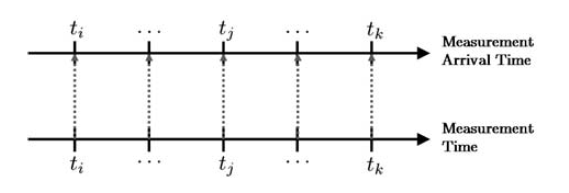
\includegraphics[width=1.0\columnwidth]{./img/undelayed_measurement.png}}
	\caption{Sequence of measurements unaffected by delay}
	\label{fig:undelayed_measurement}
\end{figure} 

\begin{figure}
	%trim={Left Bottom Right Top}
	% \fbox%
	{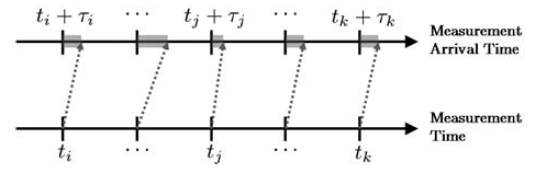
\includegraphics[width=1.0\columnwidth]{./img/delayed_measurement.png}}
	\caption{Sequence of measurements affected by delay}
	\label{fig:delayed_measurement}
\end{figure} 


 
	
\section{Notation}	\label{sect:notation}
	\cyan
This section enlists and defines the notations used in this paper.
\begin{table}[h!]
	\centering
	\begin{tabular}[h]{|c|l|}
		\hline
		x 				& non-bold face variables denote $scalars$ 			\T \\
		$\Boldx$ 		& boldface lower-case denotes $vector$ quantities	\T \\ 	
		$\BoldX$ 		& boldface upper-case denotes $matrix$ quantities	\T \\
		$\Boldx$ 		& true value of $\Boldx$ 							\T \\  	
		$\hat{\Boldx}$ 	& estimated value of $\Boldx$						\T \\	
		$\hat{\Boldx}_{k}$ & estimated value of $\Boldx$ at time step $k$	\T \\	
		$\mathbb{R}$ 	& real numbers										\T \\ 	
		$\mathbb{R}^n$ 	& $n$-tuple of reals								\T \\
		(a,$\dots$,b) 	& open interval	between $a$ and $b$					\T \\
%		$\BoldI_{a \times b}$ 	& identity matrix with $m$ rows and $n$ columns 	\T \\
		\hline
		
	\end{tabular}
	\caption{Notational conventions.}
	\label{table:notation}
\end{table}

\black

\section{Problem Statement}\label{sect:problem_statement}
	
%The overall state estimation process involves two steps, time propagation and measurement update. 
%While this article includes a linearized time propagation for the completeness of the estimation process, the prime focus shall be on the measurement update portion. 

Recursive Bayesian estimation consists of time propagation for prediction of the state and measurement update to correct the predicted state.
When there is delay in the time a sensor provides a measurement and the time it is made available for the measurement update, the estimation process need to be address the delay before incorporating the measurement into the update.
This article describes an approach to address the delay for a discrete-time estimation model.

Let $\Boldx_k \in\mathbb{R}^n$ represent the state vector at discrete-time $k$.
The measurement update at time $k$ involves a state prior and a measurement vector $\Boldy_k\in\mathbb{R}^m$.
%
The prior for the state $\Boldx_k$ is modeled as a Gaussian probability distribution $\Boldx_k \sim \mathcal{N}(\hat{\Boldx}_k^-,\BoldP_k^-)$, where the mean $\hat{\Boldx}_k^-$ and error covariance matrix $\BoldP_k^-$ are provided by the time propagation step.
  
The delayed measurement vector at time $k$ is:
\begin{align} \label{eqn:MeasurementModel}
	\Boldz_{k} = \BoldC_{k-N} \, \Boldx_{k-N} + \Boldeta_k
\end{align}
where $N$ is delay time steps, $\BoldC_{k-N}\in \mathbb{R}^{m \times n}$ is the measurement matrix and $\Boldeta_k \sim \mathcal{N}(\0,\,\BoldR)$ is white Gaussian measurement noise.

The undelayed measurement vector at time $k$ is:
\begin{align} \label{eqn:MeasurementModel}
\Boldy_k = \BoldH_k \, \Boldx_k + \Boldeta_k
\end{align}
where $\BoldH_k \in \mathbb{R}^{m \times n}$ is the measurement matrix and $\Boldeta_k \sim \mathcal{N}(\0,\,\BoldR)$ is white Gaussian measurement noise. The covariance matrix $\BoldR$ is assumed to be invertible and diagonal\footnote
{\label{ftnt:R_assumption}
	Note that there is no restriction attached to this assumption. The solution can be used for any  covariance matrix by using the transformation $\Boldy' =\BoldSigma_R  \, \Boldy$ with $\BoldR^{-1} = \BoldSigma_R \, \BoldSigma_R^\top$, the measurement model for $\Boldy'$ is:
	$$\Boldy'=\BoldH' \,\Boldx+\Boldeta' \mbox{ where } \BoldH' = \Sigma_R  \, \BoldH \mbox{ , } \Boldeta' \sim \mathcal{N}(\0,\,\BoldI).$$
} 
which can be written as $\BoldR = \sum_{i=1}^{m} \sigma_{i}^2 \, \Bolde_i  \,{\Bolde_i}^\top$, where $\Bolde_i$ is the $i^{th}$ column of the identity matrix $\BoldI \in \mathbb{R}^{m \times m}$ .
The prior and measurement noise are independent.

Some of the measurements will be affected by outliers.
Outlier measurements are those that are very unlikely given the model stated in eqn. (\ref{eqn:MeasurementModel}). 
When the $i$-th measurement is affected by an outlier, that measurement could be considered to be modeled by
\begin{equation}\label{eqn:MeasurementModel_s}
	y_i = \Boldh_i \, \Boldx + \eta_i +s_i,
\end{equation} where $s_i$ represents the outlier and $\Boldh_i$ is the $i$-th row of $\BoldH_k$; however, 
there is usually no known model for the outlier $s_i$.






\section{Estimation Using Measurement Without Delay} \label{sect:estimation_no_delayed_msr}
	In this section, state estimation using a linear Kalman filter will be described for the linear system model in eqns. (\ref{eqn:LinearStateProp}) and (\ref{eqn:LinearUndelayedMeasurement}) while assuming that delayed measurements described by eqn.(\ref{eqn:LinearDelayedMeasurement}) are absent at all times.\\
	\input{./Sections/KF_equations}	
%	\subsection{System Model}
%	The state estimation algorithm are designed using the standard state-space model:
\begin{align} \label{eqn:state_prop_model}
	\Boldx_{k+1} &\doteq \BoldF \Boldx_k + \BoldGamma \Boldw_k \\
	\label{eqn:delayed_msr_update_model}
	\Boldz_k &\doteq \BoldC_{k-N} \Boldx_{k-N} + \Boldeta_k	\\
	\label{eqn:msr_update_model}
	\Boldy_k &\doteq \BoldH_k \Boldx_k + \Boldeta_k	
\end{align} 
The rover state vector is 
\begin{equation} \label{eqn:state_vector}
	\Boldx = [\,\Boldp^\top \!\!\!, \, \Boldv^\top \!\!\!, \, \Bolda^\top \!\!\!, \, N, \, b]^\top 
	\in \mathbb{R}^{n_s}
\end{equation}
where $\Boldp$, $\Boldv$, $\Bolda$ $\in \mathbb{R}^3$ represent the rover position, velocity and acceleration, respectively. $N$ is the delay time step of secondary measurement. $b$ is the secondary measurement bias. 
Therefore, $n_s = 11$. $\BoldF \in \mathbb{R}^{n_s \times n_s}$ is the state transition matrix.
$\Boldw_k \sim \mathcal{N}(\0,\,\BoldQ)$ is the process noise vector which is assumed to have a Gaussian distribution. $\BoldGamma \in \mathbb{R}^{n_s \times n_s}$ is the corresponding noise matrix. $\tau$ and $T$ are used to denote the time increments between successive state propagation and measurement update steps. 
Since the propagation is done at higher rate compared to measurement update, $\tau \ll T$.


	

\section{Estimation Using Uncertain Time-Delayed Measurement} \label{sect:estimation_delayed_msr}	
	\begin{figure}
	{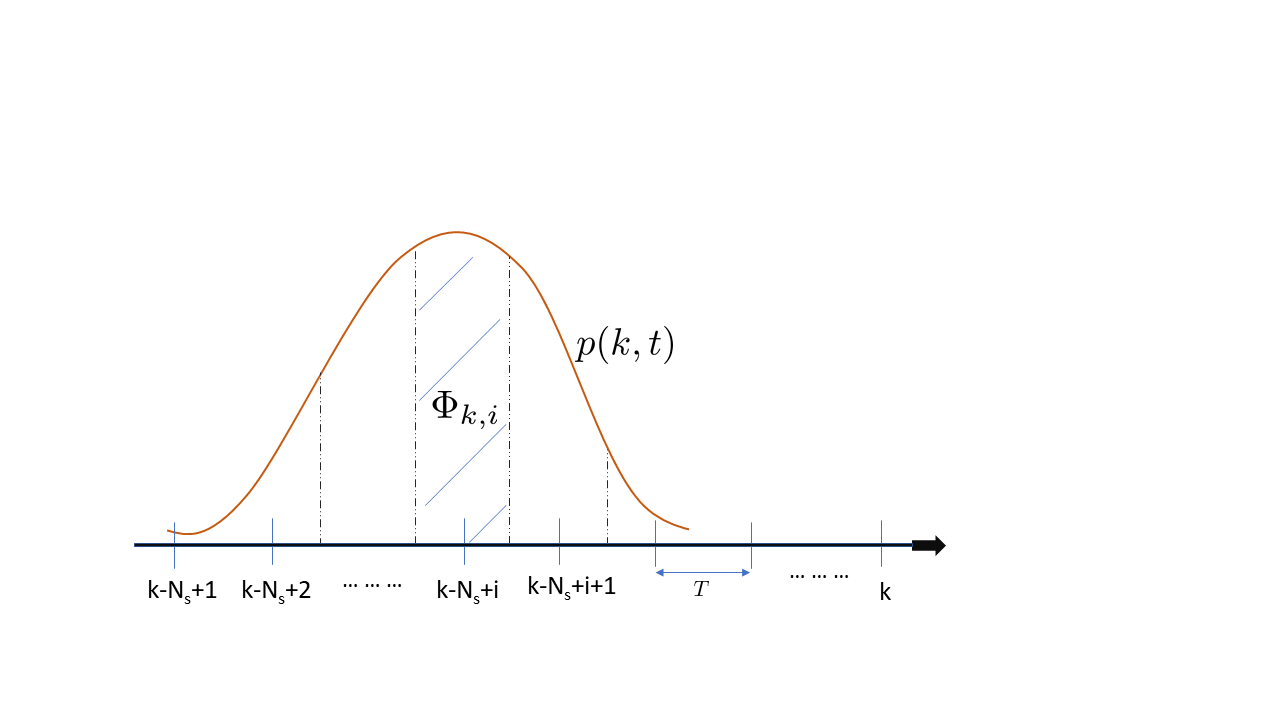
\includegraphics[width=1.0\columnwidth]{./img/delay_uncertainty.png}}
	\caption{Uncertianty of delay}
	\label{fig:delay_uncertainty}
\end{figure}

This section will describe the state estimation approach for the linear system in eqns. (\ref{eqn:LinearStateProp}) and (\ref{eqn:LinearUndelayedMeasurement}), along with time delayed measurements modelled in eqn. (\ref{eqn:LinearDelayedMeasurement}), which are corrupted by unknown bias $\Boldb_k$. 
For the derivation of the approach described in this section the reader is advised to refer to Section IV in \cite{choi2012state}.

It is essential to know the value of bias to migitate its effect on the posterior estimate of the state. Since it's not known prior to the estmiation, $\Boldb_k$ is simultaneously estimated along with the state. 
Assume that state vector at time $k$ is represented by $\Boldxi_k$.
The simultaneous estimation of the state \& the bias is achieved by performing estimation over an updated state vector defined as 
$
	\Boldx_k =
	\begin{bmatrix}
		\Boldxi_k^\top & \Boldb_k^\top
	\end{bmatrix}^\top. 
$

For the updated state vector, the linear time propagation model of eqn. (\ref{eqn:LinearStateProp}) can be rewritten as
\begin{align}
	\label{eqn:LinearStateProp4UpdatedState}
	\Boldx_{k+1} &\doteq \BoldF \Boldx_k + \BoldGamma \Boldw_k,
\end{align}

the linear measurement models in eqns. (\ref{eqn:LinearDelayedMeasurement}) and (\ref{eqn:LinearUndelayedMeasurement}) can be rewritten as
\begin{align}
	\label{eqn:LinearDelayedMeasurement4UpdatedState}
	\Boldz_k &\doteq \Big[ \BoldH_{k-N} \ \ \BoldI_{m_d} \Big] \Boldx_{k-N} +\Boldzeta_k \\
	\label{eqn:LinearUndelayedMeasurement4UpdatedState}
	\Boldy_k &\doteq \Big[ \BoldC_k \ \ \0_{m_u \times m_d} \Big] \Boldx_k + \Boldeta_k
\end{align}


The probability density function (PDF) $p(t)$ of the delay is assumed to be a known. As shown in figure (\ref{fig:delay_uncertainty}) the pdf is assumed to span over $\check{N}$ time steps. This assumption assigns a probability for correspondence of the delayed measurement $\Boldz_k$ with each of the time steps within time step $k$ and $k- \check{N}$.
Correspondence $r(k,i)$, $\forall i \in \{0, \dots, \check{N}\}$, signifies that measurement $\Boldz_k$ was induced by the state $\Boldx_{k-\check{N}+i}$.
The probability of correpondence $r_i$ is computed as
\begin{align}
	\Phi_{k,i} &= P(r(k,i)) \\
	&= P(t_l \le t \le t_u) \\
	&= \int_{t_l}^{ t_u} p(t) dt,
\end{align}
where $t_l = {j\tau - \frac{\tau}{2}}$, $t_u = {j \tau + \frac{\tau}{2}}$, $j = k - \check{N} + i $, $P(\cdot)$ denotes probability and $p(\cdot)$ denotes pdf of the time delay. When the PDF of the delay is specified, the maximum delay $\check{N}$ can be calculated using the cmulative distribution function (CDF) of the PDF. 
A value of $\check{N}$ should be chosen such that CDF of the time delay exceeds a given threshold. 
%A higher threshold value 99.6\% will ensure that the state $\Boldx_s$, where $k-\check{N} \le s \le k$, which induced the delayed measurement $\Boldz_k$ .
Choi et. al. have shown that probability of the correspondence $r_i$ for the given measurment $\Boldz_k$ is \cite{choi2012state}
\begin{align}
	P(r(k,i) | \Boldz_k ) = P(r(k,i)) = \Phi_{k,i}
\end{align}

Then, the optimal state estimator is
\begin{align}
	\hat{\Boldx}_k = \sum_{i=0}^{\check{N}} \Phi_{k,i} \hat{\Boldx}_{k,i},
\end{align}
where $\hat{\Boldx}_{k,i}$ is the estimation posterior computed the state estimate $\hat{\Boldx}_j^+$ computed in eqn. (\ref{eqn:posterior_state_estimate}), where $j = k - \check{N} + i$.

The optimal covariance matrix of the estimate is
\begin{align}
	\BoldP_k = \sum_{i = 0}^{\check{N}} \Phi_{k,i} [\BoldP_{k,i} + \hat{\Boldx}_k \hat{\Boldx}_k^\top] - \hat{\Boldx}_k \hat{\Boldx}_k^\top	
\end{align}
where $\BoldP_{k,i}$ is $a~posteriori$ state covariance matrix $P_j^+$ computed in eqn. (\ref{eqn:posterior_state_covar}),  where $j = k - \check{N} + i$. $\check{N}$




	
%	\subsection{Estimation Using Augmented State Kalman Filter }
%	The state augmentation is acheived by concatination of state vectors at time step $k$ with state at preceeding time step.
For $N$ time step delays, the agumented state vector is
\begin{align}
	\tilde{\Boldx}_k =
	\begin{bmatrix}
		\Boldx_k \\ \Boldx_{k-1} \\ \vdots \\ \Boldx_{k-N}
	\end{bmatrix} 
\end{align}


The uncertain delay parameter $\tau_k$ and the measurement bias parameter $\Boldb_k$ are unknown. Hence, the state vector is augmented with these unknown parameters to estimate their values. The augmented state is defined as
\begin{align}
	\tilde{\Boldx}_k =
	\begin{bmatrix}
		\Boldx_k \\ \tau_k \\ \Boldb_k
	\end{bmatrix} 
\end{align}
The continuous-time dynamics of the uncertain delay parameter $\tau_k$ is modelled as $\dot{\tau}(t) = \vartheta(t)$, where $\vartheta(t)$ is a white Gaussian noise. 

The discrete-time system model as a function of the augmented state is represented as
\begin{align}
	\tilde{\Boldx}_{k+1} &= 
	\tilde{\Boldf} \, \Big( \tilde{\Boldx}_k, \Boldu_k \Big) + \Boldpsi_k\\
	\begin{bmatrix}
		\Boldx_{k+1} \\ \tau_{k+1} \\ \Boldb_{k+1}
	\end{bmatrix} &= 
	\begin{bmatrix}
		\Boldf \Big( \big[\, \BoldI \ \ 0 \ \ 0 \big] \,\tilde{\Boldx}_k, \Boldu_k \Big) + \Boldomega_k \\ \vartheta_k \\ \varphi_k
	\end{bmatrix} \nonumber
\end{align}
where $\Boldpsi_k = \begin{bmatrix} \Boldomega_k^\top & \vartheta_k & \varphi_k. \end{bmatrix}^\top$

The measurements in eqns. (\ref{eqn:DelayedMeasurementModel}) \& (\ref{eqn:UndelayedMeasurementModel}) as the functions of the augmented state are represented as
\begin{align} 
	\label{eqn:DelayedMeasurementModelAug}
	\Boldz_k &= \tilde{\BoldH}_k \Big( \tilde{\Boldx}_k \Big) + \Boldzeta_k \\
	\label{eqn:UndelayedMeasurementModelAug}
	\Boldy_k &= \Boldc_k \Big( \big[\, \BoldI \ \ \0_{m_u \times m_u} \ \ \0_{m_u \times 1} \big] \,\tilde{\Boldx}_k \Big) + \Boldeta_k.
\end{align}
	

\section{Application in Gantry-Trolley Positioning}
	The solution approach described in Section \ref{sect:estimation_delayed_msr} is proposed for position estimation of a trolley mounted on a gantry crane at a container yard (shown in Figure \ref{fig:field_front_view}). 
The schematic digram in Figure \ref{fig:field_front_view} illustrates the physical setup of the gantry crane in a yard above a row of containers. 
Similarly, Figure \ref{fig:field_side_view} illustrates a side view of the yard.  
Coordinate axes of various local reference frames have been labelled. 
The relevant reference frames are Field Frame (F), Gantry Frame (G) and Trolley Frame (T).

A trolley traverses parallel to $G_x$ axis, on a rail placed on top of the gantry structre. The gantry-crane structure can travel along $F_y$ axis.

The position of the trolley is measured using two sensors: a Global Navigation Satellite System (GNSS) receiver and an encoder. 
The GNSS receiver is permanently place on top of the trolley (interchangeably also called rover) and collects raw measurements from positioning satellites to implement differential positioning.
The encoder is situated on the gantry rail and measures position of the trolley along the $G_x$ direction.

	\subsection{Rover Dynamic Model}
	At time step $k$, the system state vector is $\Boldx = [\,\Boldp^\top \dss,  \, \Boldv^\top \dss, \, \Bolda^\top \dss, t_r, \beta_r, \Boldb^\top ]^\top \in \mathbb{R}^{n_s} $, where $\Boldp$, $\Boldv$, $\Bolda$ $\in \mathbb{R}^3$ represent the rover position, velocity and acceleration, respectively.
The use of subscript to represent time step has been dropped for current section. 
%Instead it shall be used to denote a certain portion of the variable corresponding to the state variables represented by the   $\Boldx$.
The PVA state vector is $\Boldx_v = [\,\Boldp^\top \dss,  \, \Boldv^\top \dss, \, \Bolda^\top]$.
The receiver clock state vector is $\Boldx_c = [t_r, \beta_r]^\top$, where $c$, $\beta$ $\in \mathbb{R}$ are the receiver clock bias and clock drift, respectively. 
$\Boldx_b = \Boldb\in \mathbb{R}^{m_d}$ is the vector of bias affecting the delayed measurement $\Boldz$. 
Therefore, $n_s = 11 + m_d$. $\BoldF \in \mathbb{R}^{n_s \times n_s}$ is the state transition matrix.
$\Boldw \sim \mathcal{N}(\0,\,\BoldQ)$ is the process noise vector which is assumed to have a Gaussian distribution. $\BoldGamma \in \mathbb{R}^{n_s \times n_s}$ is the corresponding noise matrix. $\tau$ and $T$ are used to denote the time increments between successive state propagation and measurement update steps. 
Since the propagation is done at higher rate compared to measurement update, $\tau \ll T$.
When the GNSS pseudorange measurements are used the observation matrix $\BoldC$ is
\begin{equation}
	\BoldC = \begin{bmatrix}		
		\mathbfcal{C} & \0_{m \times 3} & \0_{m \times 3} & \1_{m \times 1} & \0_{m \times 1} \\		
	\end{bmatrix}
\end{equation}
where $\mathbfcal{C} = [\, \mathfrak{C}^1 \, \mathfrak{C}^2 \, \dots \, \mathfrak{C}^m ]^\top$ and each $\mathfrak{C}^s$ represents a line-of-sight unit vector between satellite $s$ and the rover GNSS antenna. 
The symbols $\0_{a \times b}$ and $\1_{a \times b}$ are  matrices consisting of $a$ rows and $b$ columns whose all entries are $0$s and $1$s, respectively. 

The sub-components $\Boldx_v$, $\Boldx_c$ and $\Boldx_b$ propagate independently through time hence their respective components in the state space model are not coupled.
The matrices of the discrete-time state-space model are
\begin{align} 
	\BoldF = \begin{bmatrix} \BoldF_v \dss & \0_3 \dss & \0_3 \\ \0_3 \dss & \BoldF_c \dss & \0_3 \\ \0_3 \dss & \0_3 \dss & \BoldF_b \end{bmatrix} \dss, 
	\BoldGamma = \begin{bmatrix} \BoldGamma_v \dss & \0_3 \dss & \0_3 \\ \0_3 \dss & \BoldGamma_c \dss & \0_3 \\ \0_3 \dss & \0_3 \dss & \BoldGamma_b \end{bmatrix} \dss, 
	\BoldQ = \begin{bmatrix} \BoldQ_v \dss & \0_3 \dss & \0_3 \\ \0_3 \dss & \BoldQ_c \dss & \0_3 \\ \0_3 \dss & \0_3 \dss & \BoldQ_b \end{bmatrix}
\end{align}
%The time step of state propagation is defined as $T = 0.1$ seconds and the measurement update using GNSS pseudorange occur once every 1 second.

The continuous-time PVA vehicle model is
\begin{align}
	\dot{\Boldx}_v(t) \doteq 
	\begin{bmatrix}
		\0_3 & \BoldI_3 & \0_3 \\ \0_3 & \0_3 & \BoldI_3 \\ \0_3 & \0_3 & -\lambda_a \BoldI_3
	\end{bmatrix} 
	\Boldx_v(t) +
	\begin{bmatrix} \0_3 & \0_3 & \0_3 \\ \0_3 & \0_3 & \0_3 \\ \0_3 & \0_3 & \BoldI_3 \end{bmatrix} \Boldw_a(t)
\end{align}
where $\Boldomega_a(t)$ is modeled as Gaussian white noise with power spectral density $\BoldP_a = \sigma^2_a$. 
The corresponding discrete-time description of the PVA vehicle model is approximated as
\begin{align}
	\BoldF_v &= 
	\begin{bmatrix}
		\BoldI_3 & T\,\BoldI_3 & a_3 \, \BoldI_{3} \\
		\0_3 & \BoldI_3 & a_2 \, \BoldI_{3} \\
		\0_3 & \0_3 & a_1 \, \BoldI_{3}
	\end{bmatrix}, ~ \\
	\BoldGamma_v &\approx
	\begin{bmatrix}
		\big(T^5/20 \big)^{\frac{1}{2}} \, \BoldI_3 & \0_3 & \0_3\\
		\0_3 & \big(T^3 / 3\big)^{\frac{1}{2}} \, \BoldI_3 & \0_3 \\
		\0_3 & \0_{3 \times 3} & \sqrt{T} \, \BoldI_3
	\end{bmatrix}, \\ 
	\BoldQ_{v} &= 
	\begin{bmatrix} \0_3 & \0_3 & \0_3 \\ 
					\0_3 & \0_3 & \0_3 \\
		 			\0_3 & \0_3 & \sigma^2_a \, \BoldI_3 
	\end{bmatrix},
\end{align}
where $a_1 = \exp^{\lambda_a T}$, $a_2 = (1 - \exp^{-\lambda_a T})/ \lambda_a$, and $a_3 = (\lambda_a T - 1 + \exp^{-\lambda_a T})/ \lambda_a^2$.

The continuous-time description of the clock model is 
\begin{align}
	\dot{\Boldx}_c(t) \doteq 
	\begin{bmatrix}
		0 & 1 \\ 0 & -\lambda_c
	\end{bmatrix} 
	\Boldx_c(t) +
	\begin{bmatrix} 0 \\ 1 \end{bmatrix} \Boldw_c(t)
\end{align}
where $\Boldw_c(t)$ is modeled as Gaussian white noise with power spectral density $\BoldQ_c = \sigma_c^2$. 
The corresponding discrete-time description of the clock model is 
\begin{align}
	& \BoldF_c = 
	\begin{bmatrix}
		1 & \pi_1 \\ 0 & \pi_2
	\end{bmatrix}, ~
	\BoldGamma_c \approx
	\begin{bmatrix}
		(T^3 / 3)^{\frac{1}{2}} & 0 \\
		0 & \sqrt{T}
	\end{bmatrix}, ~  
	\BoldQ_{c} = 
	\begin{bmatrix}
		\sigma_{t_r}^2 & 0 \\ 0 & \sigma_{\beta_r}^2
	\end{bmatrix}
\end{align}
where $\pi_1 = (1 - \exp^{-\lambda_c T})/ \lambda_c$ and $\pi_2 = \exp^{-\lambda_c T}$.
The approximations in $\BoldGamma_v$ and $\BoldGamma_c$ yield the correct diagonal of the discrete-time noise covariance matrix but approximates the off-diagonal terms.

The continuous-time description of the measurement bias
\begin{align}
	\dot{\Boldx}_b(t) \doteq 
	\begin{bmatrix}
		\0_3 & \BoldI_3 \\ \0_3 & -\lambda_b \BoldI_3
	\end{bmatrix} 
	\Boldx_b(t) +
	\begin{bmatrix} \0_3 & \0_3 \\ \0_3 & \BoldI_3 \end{bmatrix} \Boldw_b(t)
\end{align}
where $\Boldw_b(t)$ is modeled as Gaussian white noise with power spectral density $\BoldQ_b = \sigma_b^2$. 
The corresponding discrete-time description of the clock model is 
\begin{align}
	& \dss \BoldF_b = 
	\begin{bmatrix}
		\BoldI_3 \dss & \chi_1 \BoldI_3 \\ \0_3 \dss & \chi_2 \BoldI_3
	\end{bmatrix} \ds,
	\BoldGamma_c \approx
	\begin{bmatrix}
		\sqrt{(\frac{T^3}{3})} \BoldI_{3} \dss & \0_3 \\
		0 \dss & \sqrt{T} \BoldI_3
	\end{bmatrix} \ds,  
	\BoldQ_{c} = 
	\begin{bmatrix}
		\0_3 \dss & \0_3 \\ \0_3 \dss & \sigma_{b}^2 \BoldI_3
	\end{bmatrix}
\end{align}
where $\chi_1 = (1 - \exp^{-\lambda_b T})/ \lambda_c$ and $\chi_2 = \exp^{-\lambda_b T}$.
The approximations in $\BoldGamma_v$, $\BoldGamma_c$ and $\BoldGamma_b$ yield the correct diagonal of the discrete-time noise covariance matrix but approximates the off-diagonal terms.

\begin{table}[h!]
	\centering
	\begin{tabular}[h]{|c|c|c|c|c|c|c|c|}
		\hline
		Quantity & 	$\lambda_a$ & $\sigma_a^2$ & $\lambda_{t_r}$ & $\sigma_{t_r}^2$ & $\sigma_{\beta_r}^2$ & $\lambda_b$ & $\sigma_b^2$ \T \\ \hline
		value	 &  0.1 & 1.0 & 0.01 & 0.001 & 0 & &  \T \\ \hline
		unit	 &  $s^{-1}$ & $s^{-1}$ &  $m^2s^{-5}$ & $m^2s^{-3}$ & $m^2s^{-3}$ &  &  \T \\ \hline				
	\end{tabular}
	\caption{Parameters of the continuous-time Markov process.}
	\label{table:error_std_prediction}
\end{table}
	
	\subsection{Trolley-Gantry Physical Model}
	\begin{figure}
	{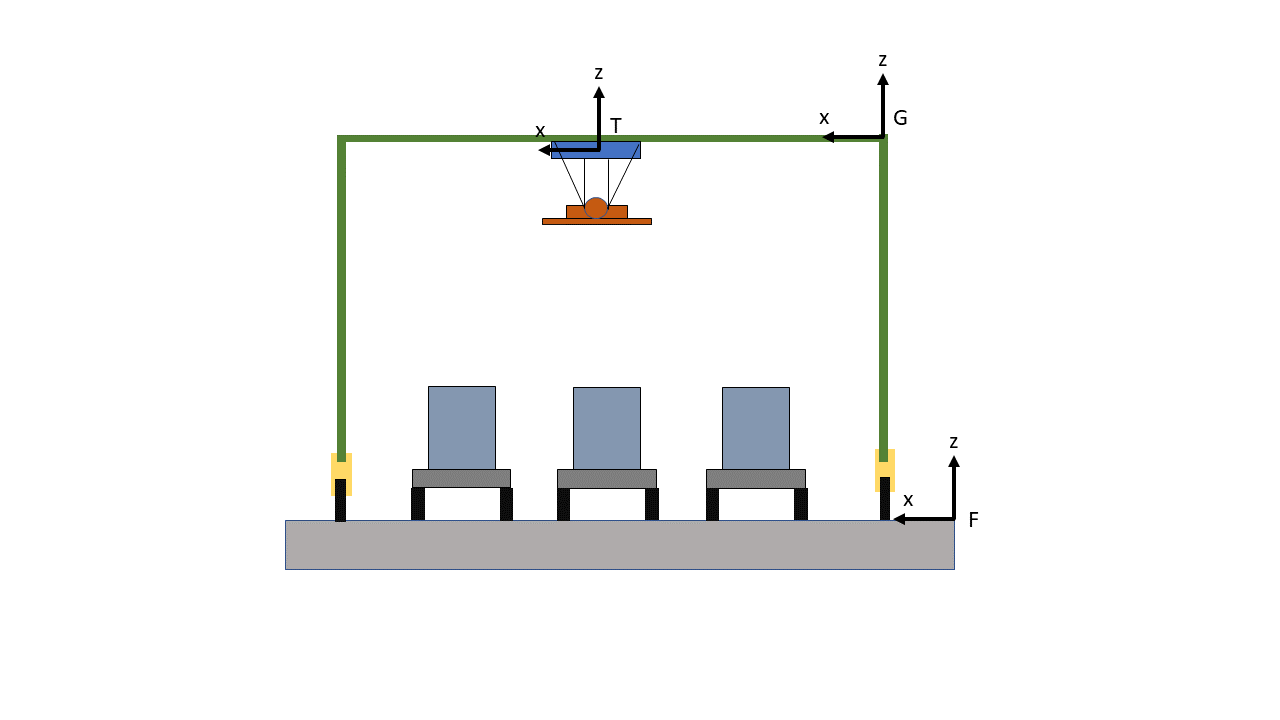
\includegraphics[width=1.0\columnwidth]{./img/field_frames1.png}}
	\caption{Front view of the container yard.}
	\label{fig:field_front_view}
\end{figure}

\begin{figure}
	{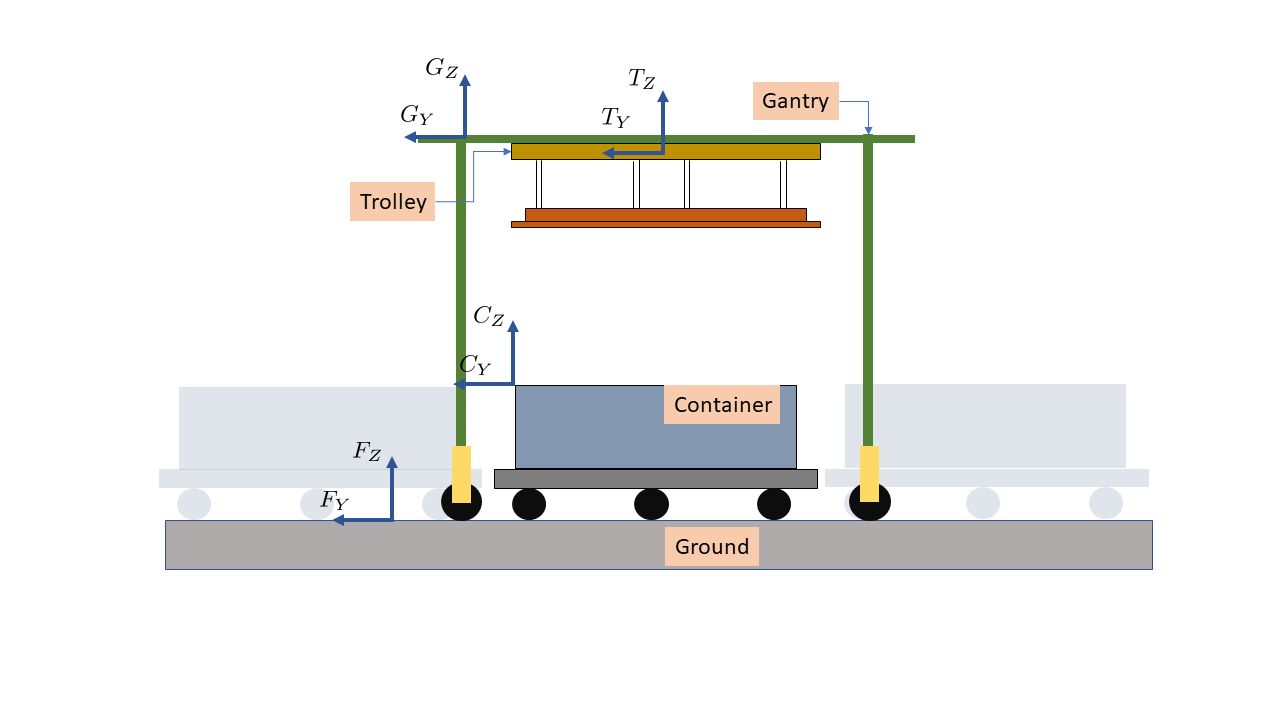
\includegraphics[width=1.0\columnwidth]{./img/field_frames2.png}}
	\caption{Side view of the container yard.}
	\label{fig:field_side_view}
\end{figure}
	

\bibliographystyle{IEEEtran}
%\bibliography{References}
\clearpage

%\appendix
%\input{./Sections/Appendix}

\clearpage


\end{document}

